\documentclass[letterpaper,10pt,titlepage,draftclsnofoot,onecolumn,onesided] {IEEEtran}
\usepackage{listings}
\usepackage{underscore}
\usepackage[bookmarks=true]{hyperref}
\usepackage[utf8]{inputenc}
\usepackage[english]{babel}
%\usepackage{titling}
\usepackage{graphicx}
\usepackage{xcolor}
\usepackage[noadjust]{cite}
\usepackage{setspace}
\nocite{*}
\graphicspath{ {img/} }
%\usepackage{abstract}

\newcommand{\namesigdate}[2][4cm]{%
  \begin{tabular}{@{}p{#1}@{}}
    #2 \\[2\normalbaselineskip] \hrule \\[0pt]
    {\small \textit{Signature}} \\[2\normalbaselineskip] \hrule \\[0pt]
    {\small \textit{Date}}
  \end{tabular}
}
\newcommand{\studentnamesigdate}[2][4cm]{%
  \begin{tabular}{@{}p{#1}@{}}
    #2 \\[2\normalbaselineskip] \hrule \\[0pt]
    {\small \textit{Signature}} \\[2\normalbaselineskip] \hrule \\[0pt]
    {\small \textit{Signature}} \\[2\normalbaselineskip] \hrule \\[0pt]
    {\small \textit{Signature}} \\[2\normalbaselineskip] \hrule \\[0pt]
    {\small \textit{Signature}} \\[2\normalbaselineskip] \hrule \\[0pt]
    {\small \textit{Date}}
  \end{tabular}
}

\hypersetup{
    bookmarks=false,    % show bookmarks bar?
    pdftitle={Progress Report},    % title
    pdfauthor={Cramer Smith, Sam Lichlyter, Eric Winkler, Zach Schneider},                     % author
    pdfsubject={Progress Report},                        % subject of the document
    pdfkeywords={IFT, Report, Postal}, % list of keywords
    colorlinks=true,       % false: boxed links; true: colored links
    linkcolor=black,       % color of internal links
    citecolor=black,       % color of links to bibliography
    filecolor=black,        % color of file links
    urlcolor=blue,        % color of external links
    linktoc=page            % only page is linked
} 

\lstdefinestyle{customperl}{
  belowcaptionskip=1\baselineskip,
  breaklines=true,
  frame=L,
  xleftmargin=\parindent,
  language=Perl,
  columns=fullflexible,
  showstringspaces=false,
  basicstyle=\footnotesize\ttfamily,
  keywordstyle=\bfseries\color{green!40!black},
  commentstyle=\itshape\color{purple!40!black},
  identifierstyle=\color{blue},
  stringstyle=\color{orange},
  numbers=left
}
\lstset{escapechar=@, style=customperl}

% Document Title:
\def\doctitle{A Tool to Visualize the Structure of a Codebase Using Information Foraging Theory Design Patterns}
\def\doctype{Progress Report}
\def\doctype{Spring Midterm Update}
\def\team{Team Postal | Group \#38}

\markboth{Oregon State University}{\doctitle}

\begin{document}

\title{\Huge{\bfseries{\textsf{\doctitle}}}\\\textsf{\Large{\doctype}}\\\textsf{\large{\team}}}
\author{Cramer Smith, Sam Lichlyter, Eric Winkler, Zach Schneider}

\maketitle
\vfill

\setlength\parindent{0pt} \textbf{Abstract:} Developer tools are often complex pieces of software. 
Gathering and manipulating useful information for a programmer can often be a slow and costly process. 
By implementing Information Foraging Theory design patterns in the creation of these tools, the information collected may be more useful or produced faster. 
Information Foraging Theory is the theory and math behind the choices people make to maximize the value of the information they find versus the cost of getting that information.
The aim of this project is to develop a tool that will act as a proof of concept to this idea and increase developer efficiency.
Through the implementation of multiple IFT design patterns, the Postal team will create a developer tool that helps enforce and maintain code structure. 

\vfill

\pagebreak

\tableofcontents


\pagebreak

\section{Project Purpose and Goals}
Developer tools are often complex pieces of software. 
Gathering and manipulating useful information for a programmer can often be a slow and costly process. 
By implementing Information Foraging Theory design patterns in the creation of these tools, the information collected may be more useful or obtained faster. 
Information Foraging Theory (IFT) is the theory and math behind the choices people make to maximize the value of the information they find versus the cost of getting that information.
The aim of this project is to develop a tool that will act as a proof of concept for IFT and increase developer efficiency.

Our project (code-named "Postal") is an extension for Visual Studio Code. 
It is being designed to allow developers to more quickly search through and better visualize their projects.
This extension will also help developers create clearer and cleaner code structure by offering reminders and suggestions about the best coding practices in the programming language they are currently using.
Any major errors or incompatibilities within the project or its files will be reported to the developer as well.

\section{Current Status}
	\subsection{Project Status}
	As of the end of week 6 of Spring term, all requirements of our project have been met, the extension itself is fully functional and most bugs in the codebase have be either resolved or negated.
	Our extension is available for download and installation from the Microsoft Visual Studio Marketplace and is labeled as our 1.0 release. 
	Previous alpha and beta versions had been available on the Marketplace but lacked some of the final functionality or had significant bugs present.
	Project Postal works and has been tested on all 3 major OS platforms, Windows 7/10, MacOS and Ubuntu specifically.
	The extension can parse and visualize most major programming languages, having been tested primarily on C, C++, HTML, CSS, JavaScript, TypeScript and PHP.
	Default grammars (a series of regular expressions that search for language-specific keywords or tags) that allow the parser to process and visualize most of these languages have been included with the extension installation.
	The program is highly extensible, allowing any user to add to existing language grammars or create new languages grammars themselves.
	To this effect, the team intends to demonstrate Project Postal at the Engineering Expo with grammars not included in the default installation, so as to show how grammars can be designed toward specific codebases.
	
	Two deficiencies of note remain in our project that were not able to be resolved by the week 5 code freeze: a separate Node.js installation and minor visualization bugs.
	At this time, the Postal Extension requires Node to be independently installed on the user's machine in order to work. 
	The reason for this additional installation requirement is that our display and window system, Electron, is too large of a package to be bundled in with a Visual Studio Code extension.
	As such, the user has to use Node's 'npm install' command to acquire Electron separately.
	The other remaining bug of note in our project is an occasional inconsistency in how a given codebase is visualized.
	Postal uses the Vis.js package to create a network of interactive visual nodes that represent files in the user's codebase.
	Occasionally, Vis will generate a network that has some file nodes set to display in a location far from the rest of the network.
	This visualization bug can typically be overcome by either redrawing the network (a button available to the user) or closing and reopening the Electron window.
	The team was not able to determine the cause of this problem, but we feel it does not significantly detract from the overall functionality of the program.
	
	\subsection{Testing Status}
	According to our agreement with our client, Prof. Chris Scaffidi, the team will conduct user testing to demonstrate whether the IFT principles with which the program was designed are effective.
	The team has both written up a series of tasks for a set of users to perform with and without the Postal Extension, as well as a post-testing questionnaire that will gauge the whether the users felt the extension helped them achieve the tasks faster or more effectively.
	These tasks and the questionnaire were both approved by our client and have been submitted to the university's Institutional Review Board (IRB) for human subject research approval.
	As of the end of week 6 of Spring term, the team is still waiting for response from the IRB.
	When approval is received, the team and our client will set up a selection of users to test our program.
	The actual testing procedures have been defined in the User Testing section later in this document.
	
\section{Remaining Work}
	\subsection{Postal Extension}
	While Functionally complete, these are several minor features the team is planing on implementing before user trails begin. 
	The first being a simple reset button built into the extension UI. 
	This will reset the state of the vis.js map to its initial positions to be used in the event of buggy behaviour or as a quick way to collapse all sub nodes.
	Additionally we would like to implement functionality that starts all files within a visualized directory collapsed into a directory.
	Currently, directory nodes are not collapsible but really should be.
	One final change to make in the extension is a fix involving file links. 
	Occasionally when a user rapidly expands nodes and enables/disable the file link button, the file links may become broken.
	While we haven't been able to find the exact cause of this bug, we plan on fixing it in time for testing.
	\subsection{User Testing}
	A large portion of work that is still in progress is user testing. 
	We are currently tuning our test questions in preparation for human trials within the next few weeks.
	Several members of the group have done trial runs with our current test questions to get feedback before the actual tests begin.
	So far the trials have been useful in finding problems with the exams and we plan on continuing to tune until we get approval from our client to begin human trials.
	After human trials, we will potentially be responsible for writing up our findings in a publishable format which may take a significant amount of time.
\section{Problems and Solutions}
	\subsection{Fall Term}
	\subsection{Pre-Week 3}
	The beginning of our project was back in August when Sam told the rest of the team about an opportunity that he had to work with Prof. Chirs Scaffidi on a senior design project. 
	The members of the team all jumped on the opportunity to work together for a professor all of us had had previously and throughly enjoyed.
	Prof. Scaffidi tasked the team with coming up with project proposals.
	The only requirements for the project is that it had to be a tool that used information foraging theory to do anything.
	The first problem was that none of the team knew what IFT was so the team took a week to brainstorm seperately and research IFT and come up with project ideas.
	After that week the team met and decided on two ideas to give to the client.
	Scaffidi chose a code base organization tool that would be an extension for Visual Studio Code.
	
	\subsection{Week 3}
	After the first couple weeks of class while other teams were just meeting the Postal team was able to start meeting and thinking about functionality as well as begin to work on the problem statement.
	The problem statement was the first document of the project and it was a challenge to create an official document and learn how to use the IEEE standard. 
	This problem was not really solved.
	The team ended up creating what they thought was a good document, and there was feedback on the document that came later in the quarter helped tremendously for the next draft of the document.
	
	\subsection{Week 4}
	During the fourth week, our client had challenged the team with accelerating the development process past the class.
	In response to this request the team started developing basic "hello world" extensions with very limited to no functionality.
	These programs served as a learning experience for the team as we develop more complex extensions these examples gave us a framework of understanding of what the code of an extension looks like.
	These small programs were good but not up to par with our clients expectations.	
	
	\subsection{Week 5}
	In week five the team revised the problem statement.
	This task was fairly easy as the team had received feedback on the first draft and therefore had a knowledge of what was expected of them.
	This week we also started work on the Requirements Document. 
	The requirements document was much more daunting than the problem statement as it was more technical, and made the team think more the project as a piece of software an not just a problem to be solved.
	The team wrote a first draft of the requirements document and made a plan to finish it the next week.
	
	\subsection{Week 6}
	With the completion of the requirements document the team had some solid ideas as to what the project was going to look like.
	This was a big step forward for the project as the team had only a fuzzy idea as to what the project really looked like at this moment.
	Now the team knew that it was going to be a web development tool instead of a general code organizer.
	This was great for the development of the project, but this narrowing of scope was not communicated to the client. 
	The team thought that they had communicated this in a meeting but apparently either our client did not understand or the idea was not stated clearly.
	This caused problems later in the process.
	
	\subsection{Week 7}
	This week we thought was a big step for the team. 
 	By this time there was a working prototype of the user interface, and a simple parser for HTML.
	The only thing was that these programs were not actually a Visual Studio Code extension but separately compiled programs.
	The team needed to figure out how to combine the program UI with Visual Studio Code.
	
	\subsection{Week 8}
	The eighth week the team finished the tech document.
	The tech document made the team look at alternatives for parts that each member had decided to focus on.
	This was eye opening as we researched alternatives to pieces of the project that the team members had never thought of before.
	
	\subsection{Week 9}
	This week was Thanksgiving week. 
	With the extra time Sam and Eric were able to further the prototype and make some small improvements.
	These small improvements still had not added the UI to the extension but the team thought that it would be good enough to show to the client. 

	\subsection{Week 10}
	Week ten was a big week as the design document was due that week. 
	This document proved to be the most confusing as the team had a particularly difficult time figuring out the IEEE standard of the software design document. 
	The team was able to struggle through the design document and create what the team thought was good document. 
	The team also was able to show to the client what we had done with the prototype so far. 
	The client was happy with the prototype, but encouraged the team to reconsider the reduction in scope that had occured previously.
	This will be factored into the work going forward.
	
	\subsection{Winter Term}
	
	
	\subsection{Spring Term}
	\subsection{Week 1}
	A meeting with our client did not go well. 
	His feelings were that the UI was not refined enough and he was disappointed that we had not been using the tool ourselves.
	We immediately shifted focus onto our UI and wrote grammars for TypeScript.
	He was much happier by our next meeting and work continued in preparation for user testing.
	\subsection{Week 4}
	Changes made to the team's expo poster board were not up to specification and needed to be reverted.
	Additionally, the team has had trouble getting the extension package to be uploaded to the Postal Market Place.
	Cramer is currently trying to find the issue and has put in a ticket with the developers for help.
	\subsection{Week 5}
	The team has made some changes to the user trials sent to our client but we have been having a little bit of trouble finding qualified pre-test subjects.
	To fix this the team simply began asking more class mates and other senior project teams for help.
	\subsection{Week 6}
	This week the team began doing trial runs in preparation for human trials.
	This led to the discovery of several minor problems with our test cases.
	First, both of our tests were being completed with about five minutes left on the timer.
	Because of that, we are not able to really determine if using our tool significantly increases the speed that a user can find information.
	To fix this, the team will increase the length of the test.
	Additionally, we discovered that we had not written all of the grammars necessary to run one of the test cases. 
	the team has resolved this by writing those grammars.
	Finally, the team also noticed that a question asked about finding the number of TODOs in a directory that did not have any, resulting in some confusion.
	The team made adjustments to fix this.
	
\section{User Testing}
	

	\subsection{Testing Description}
	%Include our actual updated user questions, brief description of test projects, what we have users do
	The test in its current state contains two sets of tasks that go with two specific software projects. 
	One is a C++ project and the other is a HTML and PHP project. 
	Both of these projects are about the same size and are of similar complexity. 
	The test subjects will go through the projects completing the tasks that we have designed to measure the effectiveness of the use of IFT. 
	\\
	The tasks are as follows: 
	
	For the \textbf{C++ project}
	\begin{enumerate}
		\item Locate the line at which void RenderingDirector::rdRender() is defined. 
		\item Find the number of functions in the snake.cpp file.
		\item There is a function that is defined in Snake.cpp, but is never used. Name that function.
		\item Find all the TODO comments in the program.
		\item Identify the return type of the Snake::Turn function.
		\item Find the number of times the Food class referenced in the gameplay-director.cpp file.
		\item Find the number of .h files included in main.cpp.
		\item Locate the file in which the Punish() function is defined.
	\end{enumerate}
	
	For the \textbf{HTML and PHP project}
	\begin{enumerate}
		\item ?index.php? is the homepage for this web application. Over time, various features and pages were added and removed. This resulted in some files that exist within the directory that have been deprecated (they are not used within the index page or any of the pages linked to index.php). Locate all the files that are deprecated. (select all that apply check list)

		\item Find the number of ?div?s in header.php
		\item Some website applications make use of several external references like jQuery and Bootstrap. Find all external references used in the project directory. (External references are links to outside resources that are not included within the project directory, and are hosted on external servers)

		\item What file and line number is ?site-menu? declared in?
		\item How many references are there to ?stylesheet.css? in the project?
		\item How many images are linked in the entire project?
	\end{enumerate}
	
	\subsection{Measuring Results}
	We will measure how long it takes the tester to complete the tasks as well as how well they answer the questions as a percentage. 
	For example if a user were to find all the TODOs they would receive a 100\% for that question. 
	If they missed one of the ten they would get a 90\%.
	If the subject failed to find any of the TODOs they would receive a 0\% for that problem.

	We will also do a post test questionnaire. 
	The questionnaire will pose the subject with a number of questions that the subject can answer on a spectrum from strongly agree to strongly disagree.

	The questionaire is as follows: 
	
	\begin{enumerate}
		\item I could effectively complete the tasks and scenarios using the Postal tools.
		\item I was able to complete the tasks and scenarios quickly using the Postal tools.
		\item The organization of information and interface elements of the Postal tools within Visual Studio Code was clear.
		\item It was easy to use this tool.
		\item I would use Visual Studio Code again.
		\item I could think of multiple scenarios for using for the Postal tool. 
		\item I would use the Postal tools within Visual Studio Code again.
		\item Seeing a project visually was useful. 
		\item I felt the file link feature$^1$ allowed me to complete the tasks more quickly.
		\item I felt the file link feature$^1$ allowed me to answer the questions with more confidence.
		\item I felt the expand feature$^2$ allowed me to complete the task more quickly.
		\item I felt the expand feature$^2$ allowed me to answer the questions with more confidence.
		\item I felt the notification feature$^3$ allowed me to complete the task more quickly.
		\item I felt the notification feature$^3$ allowed me to answer the questions with more confidence.	
	\end{enumerate}

	[1] File link feature: Internal references to other files displayed as red lines within the node network.

	[2] Expand feature: A right-click on any file node expanded the node network to include all sub-nodes (classes, functions, divs, etc.) of the indicated node.

	[3] Notification feature: Notifications (regarding malformed code, incorrect styling, etc.) were indicated by a red circle attached to the associated files/nodes and described in the notification window on the right-hand side of the screen.

	The questionnaire will help us to measure how the user feels about the usefulness and general feel of the extension. 
	The more that they strongly agree with the statements that will mean that the users enjoy and feel that the extension is useful.

	\subsection{Report Rough Draft: Information Foraging Theory Improving the Rate of Information Gain in Software Development}
	A report of the results of the an attempt to use of IFT properties used to help improve the efficiency of software development through the use of visualization. This report will describe the idea of information foraging theory as well as the Postal Extension that was developed to test the use of IFT with developers. The report will also detail the way that the software was tested along with the results of the tests, and the conclusion that is gathered from the tests. 
	
	\subsubsection{Information Foraging Theory}
	Information Theory is the idea of turning information into weighted directed graphs and then implementing these graphs to better access the data.
	
	\subsubsection{The Postal Extension}
	Postal is a proof of concept using IFT design patterns to present data to the user will improve the rate that the user can locate and navigate the information.
	We hypothesize that the use of IFT in the Postal Extension will prove to increase the productivity and efficiency of programmers navigating around code and locating different parts of the code.  
	
	\subsubsection{Experiment Procedure}
	\begin{enumerate}
		\item	In a computer Lab with 15 computers set up the extension on the 15 computers.
		\item	On the 15 computers load up the 2 testing projects.
		\item	On the 15 computers set up a document with the question that they will be answering.
		\item	Have the subjects each sit at a different computer and give them a 5 minute tutorial on the Postal Extension and how to use it.
		\item	Direct the subjects to the questions that they are answering and the project that they are answering the questions about
		\item	Give the users ten minutes to complete the set of questions.
		\item	At the end of the ten minutes direct the users to the next set of questions and the other project. 
		\item 	Give them another 10 minutes to answer the question without the use of the extension.
		\item	Once the ten minutes are over they will be given a short survey. 
		\item	The subjects will have 5 minutes to answer the survey.
		\item	Once they are done, ask that group to leave and bring in the other 15 subject and repeat the same procedure but switch the project that the subjects use the extension on. 
		\item 	Collect results.
	\end{enumerate}
	
	The tasks are as follows: 
	
	For the \textbf{C++ project}
	\begin{enumerate}
		\item Locate the line at which void RenderingDirector::rdRender() is defined. 
		\item Find the number of functions in the snake.cpp file.
		\item There is a function that is defined in Snake.cpp, but is never used. Name that function.
		\item Find all the TODO comments in the program.
		\item Identify the return type of the Snake::Turn function.
		\item Find the number of times the Food class referenced in the gameplay-director.cpp file.
		\item Find the number of .h files included in main.cpp.
		\item Locate the file in which the Punish() function is defined.
	\end{enumerate}
	
	For the \textbf{HTML and PHP project}
	\begin{enumerate}
		\item ?index.php? is the homepage for this web application. Over time, various features and pages were added and removed. This resulted in some files that exist within the directory that have been deprecated (they are not used within the index page or any of the pages linked to index.php). Locate all the files that are deprecated. (select all that apply check list)
		\item Find the number of ?div?s in header.php
		\item Some website applications make use of several external references like jQuery and Bootstrap. Find all external references used in the project directory. (External references are links to outside resources that are not included within the project directory, and are hosted on external servers)
		\item What file and line number is ?site-menu? declared in?
		\item How many references are there to ?stylesheet.css? in the project?
		\item How many images are linked in the entire project?
	\end{enumerate}
	
	\subsubsection{Measuring Results}
	We will measure how long it takes the tester to complete the tasks as well as how well they answer the questions as a percentage. 
	For example if a user were to find all the TODOs they would receive a 100\% for that question. 
	If they missed one of the ten they would get a 90\%.
	If the subject failed to find any of the TODOs they would receive a 0\% for that problem.

	We will also do a post test questionnaire. 
	The questionnaire will pose the subject with a number of questions that the subject can answer on a spectrum from strongly agree to strongly disagree.

	The questionaire is as follows: 
	
	\begin{enumerate}
		\item I could effectively complete the tasks and scenarios using the Postal tools.
		\item I was able to complete the tasks and scenarios quickly using the Postal tools.
		\item The organization of information and interface elements of the Postal tools within Visual Studio Code was clear.
		\item It was easy to use this tool.
		\item I would use Visual Studio Code again.
		\item I could think of multiple scenarios for using for the Postal tool. 
		\item I would use the Postal tools within Visual Studio Code again.
		\item Seeing a project visually was useful. 
		\item I felt the file link feature$^1$ allowed me to complete the tasks more quickly.
		\item I felt the file link feature$^1$ allowed me to answer the questions with more confidence.
		\item I felt the expand feature$^2$ allowed me to complete the task more quickly.
		\item I felt the expand feature$^2$ allowed me to answer the questions with more confidence.
		\item I felt the notification feature$^3$ allowed me to complete the task more quickly.
		\item I felt the notification feature$^3$ allowed me to answer the questions with more confidence.	
	\end{enumerate}

	[1] File link feature: Internal references to other files displayed as red lines within the node network.

	[2] Expand feature: A right-click on any file node expanded the node network to include all sub-nodes (classes, functions, divs, etc.) of the indicated node.

	[3] Notification feature: Notifications (regarding malformed code, incorrect styling, etc.) were indicated by a red circle attached to the associated files/nodes and described in the notification window on the right-hand side of the screen.
	
	\subsubsection{Conclusion}
	
	We will write this once we get the results of the project.	


\pagebreak	
\section{Images}
	\begin{figure}
		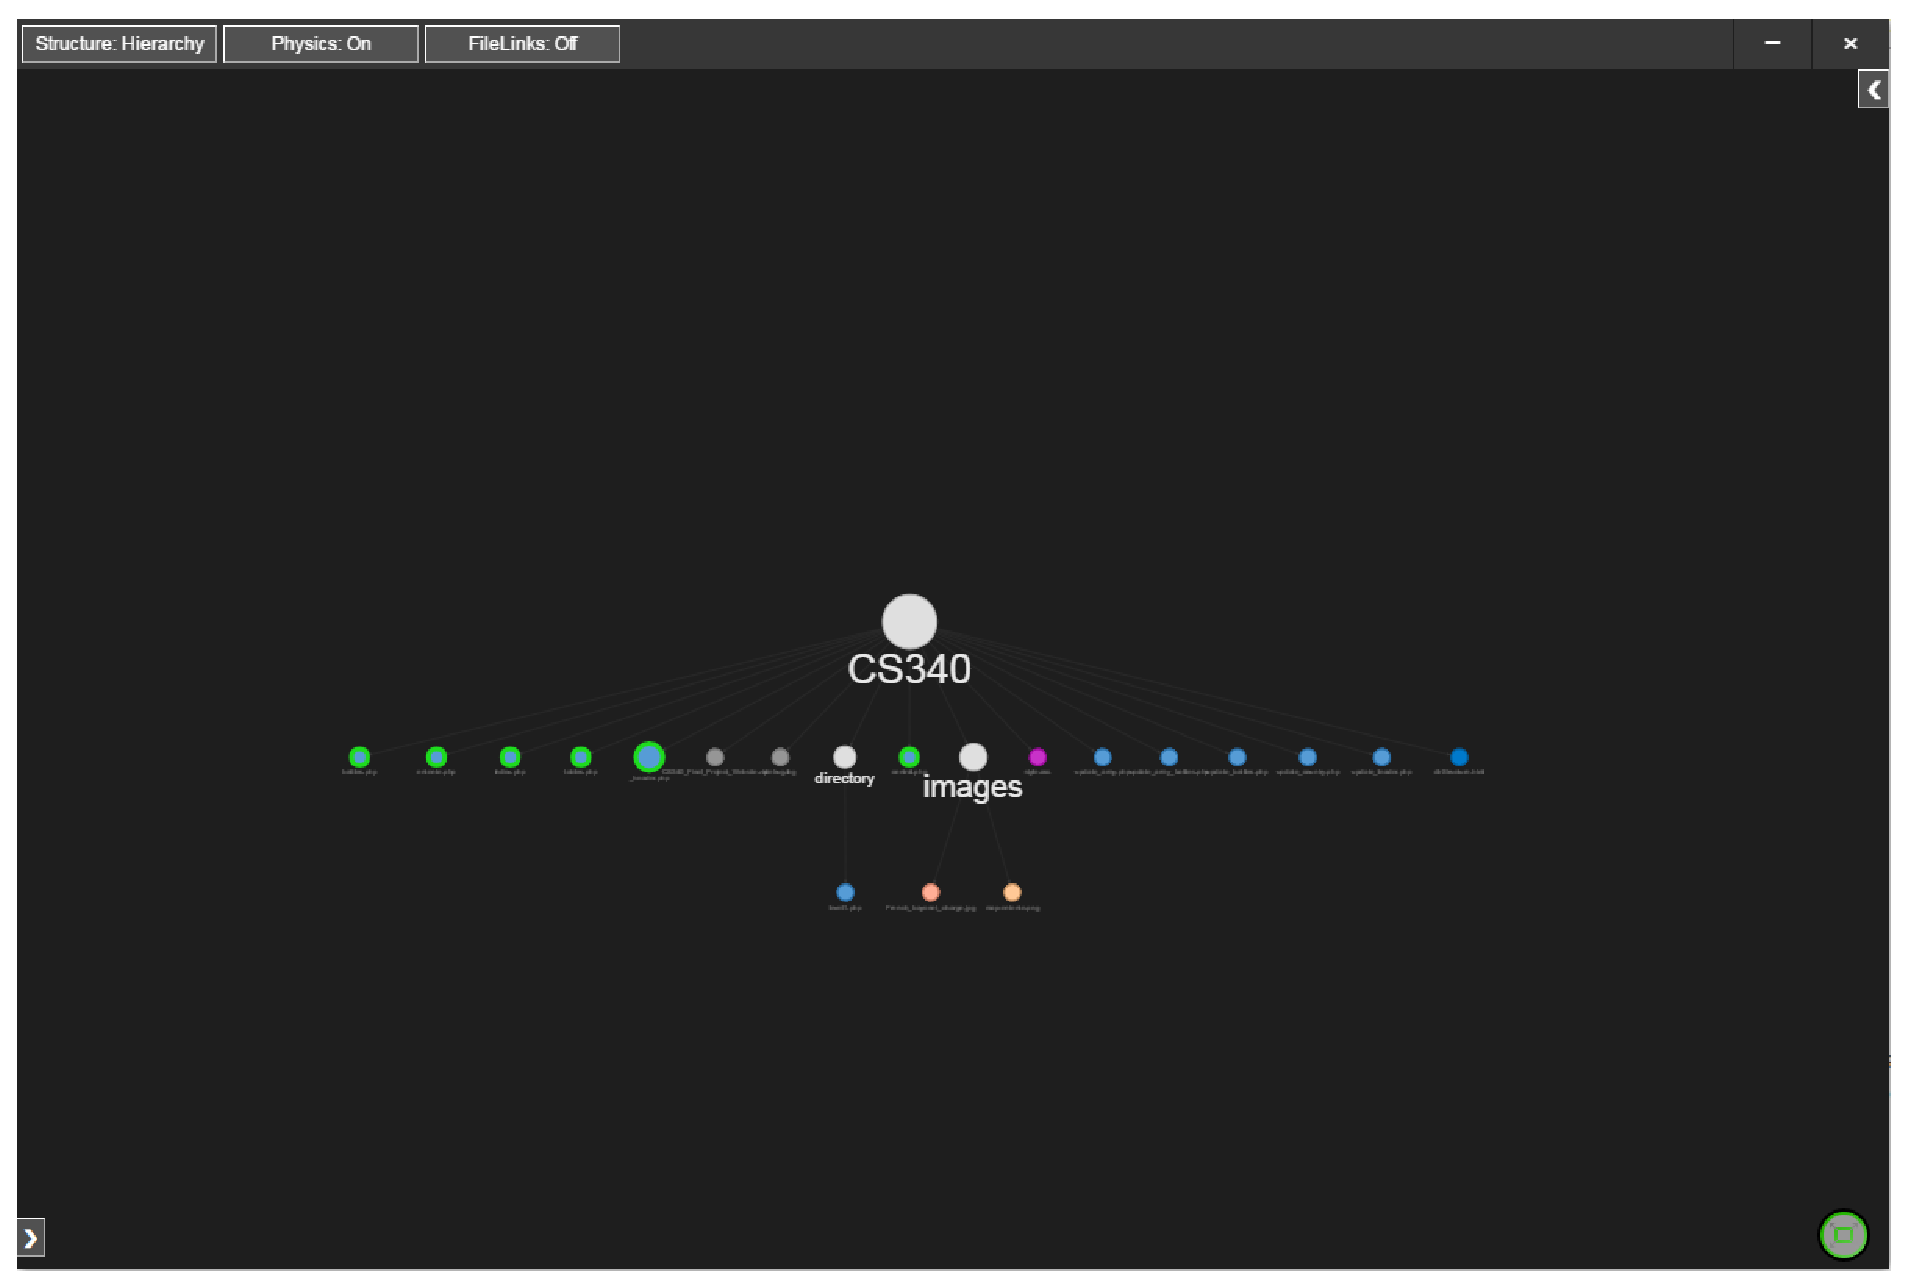
\includegraphics[width=400px]{PostalUI}
		\caption{Visualization Interface}  
	\end{figure}
	
	\begin{figure}
		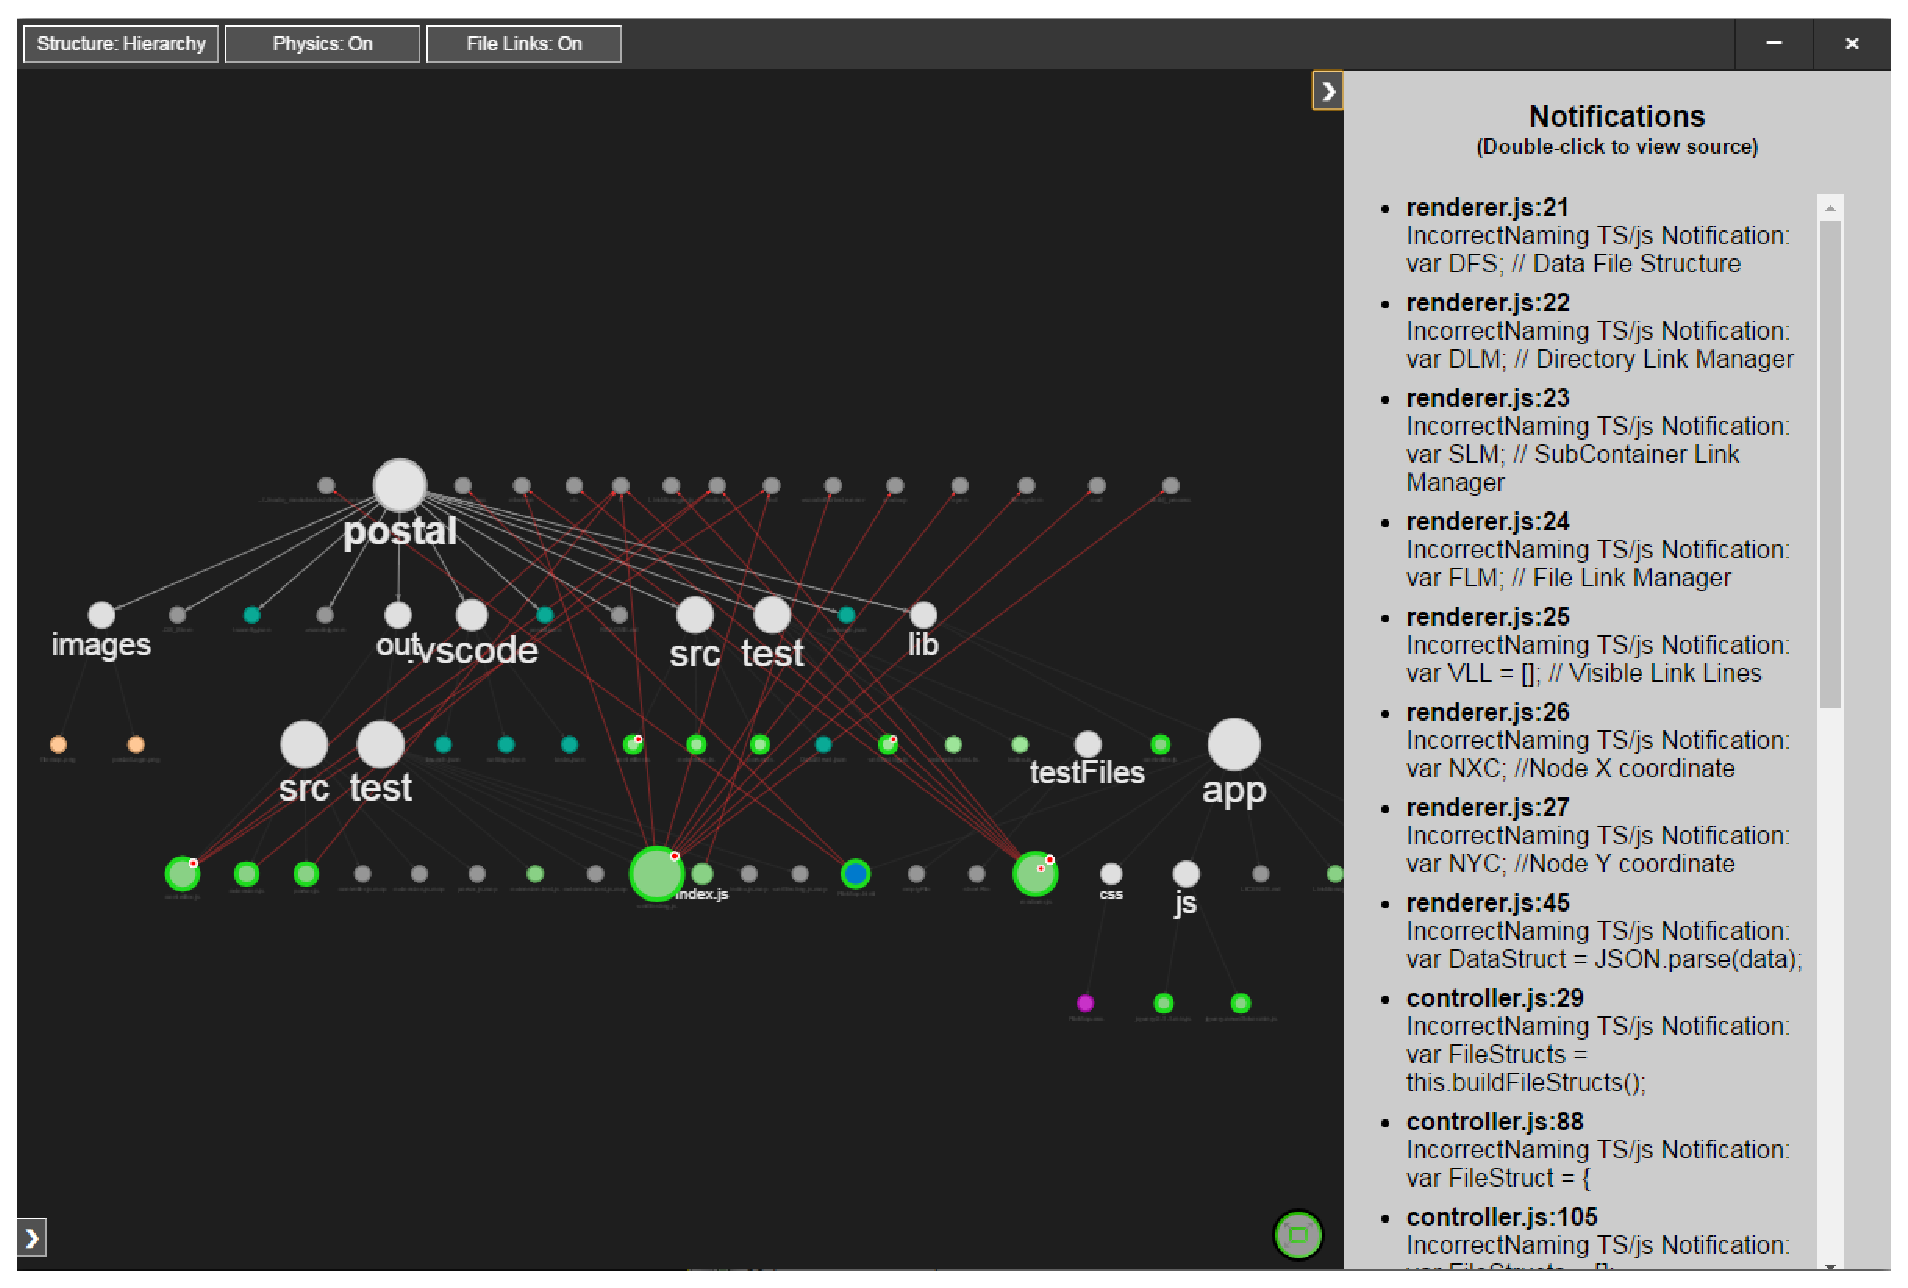
\includegraphics[width=400px]{PostalNotification}
		\caption{Notification Interface}  
	\end{figure}
	
	\begin{figure}
		\includegraphics[width=400px]{UpdatedDataStruct}
		\caption{Updated Data Structure}
	\end{figure}

\pagebreak
\section{Code Samples}
	\subsection{Example Grammar}
	This is the default grammar that parses HTML and PHP files for divs and links.
	
	\begin{lstlisting}
{
    "id" : 0,
    "title" : "html",
    "filetypes" : ["html", "php"],
    "rules" : [{
            "title": "div",
            "type": "tagged",
            "options" : {
                "tagStart": "<div",
                "namedOption" : "id=\"(.+?)\"",
                "tagEnd": ">",
                "closingTag": "</div>",
                "nodeColor": "blue"
            }
        }, {
            "title": "href link",
            "type" : "link",
            "options" : {
                "link": "href=[\"](.+?)[\"]",
                "nodeColor": "blue"
            }
        }, {
            "title": "includes link",
            "type": "link",
            "options": {
                "link": "include=[\"](.+?)[\"]",
                "nodeColor": "blue"
            }
        }, {
            "title": "body",
            "type": "tagged",
            "options" : {
                "tagStart": "<body",
                "tagEnd": ">",
                "closingTag": "</body>",
                "nodeColor": "blue"
            }
        }
    ]
}
	\end{lstlisting}

	\pagebreak
	\subsection{Recursive Get All Links}
	This function grabs all the links from the data structure of a specified file struct and it's children.
	\begin{lstlisting}
// Recursive function to get all links from this and children
function getAllLinksFromFileStructRecursive(FileStructID) {
    var links = [];

    // check parent
    if (DFS[FileStructID].links.length > 0) {
        for (var i = 0; i < DFS[FileStructID].links.length; i++) {
            var link = DFS[FileStructID].links[i];
            links.push(link);
        }
    }

    // check children
    if (DFS[FileStructID].subContainers.length > 0) {
        var childLinks = [];
        for (var i = 0; i < DFS[FileStructID].subContainers.length; i++) {
            var childFileStructID = DFS[DFS[FileStructID].subContainers[i].toFileStructid].id;
            childLinks = getAllLinksFromFileStructRecursive(childFileStructID);

            // push what we found to parents link list
            for (var j = 0; j < childLinks.length; j++) {
                links.push(childLinks[j]);
            }

        }
    } 

    return links;
}
	\end{lstlisting}

\pagebreak
\bibliographystyle{IEEEtran}
\bibliography{progress-report-team38}


\end{document}

